\documentclass{article}
\usepackage{aaai}
\usepackage{graphicx}

% Big margins for now so people can take notes/scribbles.
%\usepackage{fullpage}

\title{Parallel Best NBlock First}
\author{Ethan Burns \and Seth Lemons \and Wheeler Ruml \\
Department of Computer Science \\
University of New Hampshire \\
Durham, NH 03824 USA \\
\{eaburns,seth.lemons, ruml\}@unh.edu}
\date{\today}

\begin{document}
\maketitle

\begin{abstract}
We are approaching a time when it will no longer be beneficial for
hardware manufactures to create micro-processors with greater clock
speeds.  In order to get increased performance, software developers
will need to take advantage of concurrency and multi-core processors.
We propose a best-first search algorithm which makes use of multiple
core CPUs in order to more quickly solve search problems which are
small enough to fit into memory.  We propose a new algorithm called
Parallel Best NBlock First (PBNF) for performing a parallel best-first
style heuristic search.
\end{abstract}

\section{Introduction}

As microprocessor manufacturers build processors with more and more
cores, software developers are being pressured to create algorithms to
make better use of the newly available parallelism.

\section{Background}

\subsection{Structured Duplicate Detection}

In \cite{zhou:sdd} Zhou and Hansen propose a new method for external
memory graph search called Structured Duplicate Detection (SDD).  SDD
uses a projection function, which is a many-to-one mapping from states
in the search space to states in an abstract space, to decompose a
search graph.  The projection function creates an abstract state-space
of nodes that are the projections of nodes in the original state
space.  An abstract node $y$ is said to be the \emph{image} of a node
$x$ if $p(x) = y$ for a projection function $p$.  Likewise, the node
$x$ is said to be a \emph{pre-image} of an abstract node $y$ if $p(x)
= y$.  Additionally an abstract node $y'$ is a successor of an
abstract node $y$ if there are two states $x$ and $x'$ such that $x'$
is a success of $x$, the projection of $x$ is $y$ and the
projection on $x'$ is $y'$.  In other words:

\begin{eqnarray*}
&&x' \in successors(x) \wedge p(x) = y \wedge p(x') = y' \\
&\Rightarrow& y' \in successors(y)
\end{eqnarray*}

The term \emph{nblock} is used to refer to all nodes in the state
space that map to the same projected node.  Zhou and Hansen show that
when performing duplicate detection, only nodes in the same nblock
must be checked for duplicates.  They also show that children of a
node $x$, whose image is $y$, will only fall into the nblocks that
correspond to abstract states that are successors of $y$.  This set of
nodes is called the \emph{duplicate detection scope} of the abstract
node $y$.

\begin{figure}
\begin{center}
\includegraphics[width=2in]{images/tile-abstraction.eps}
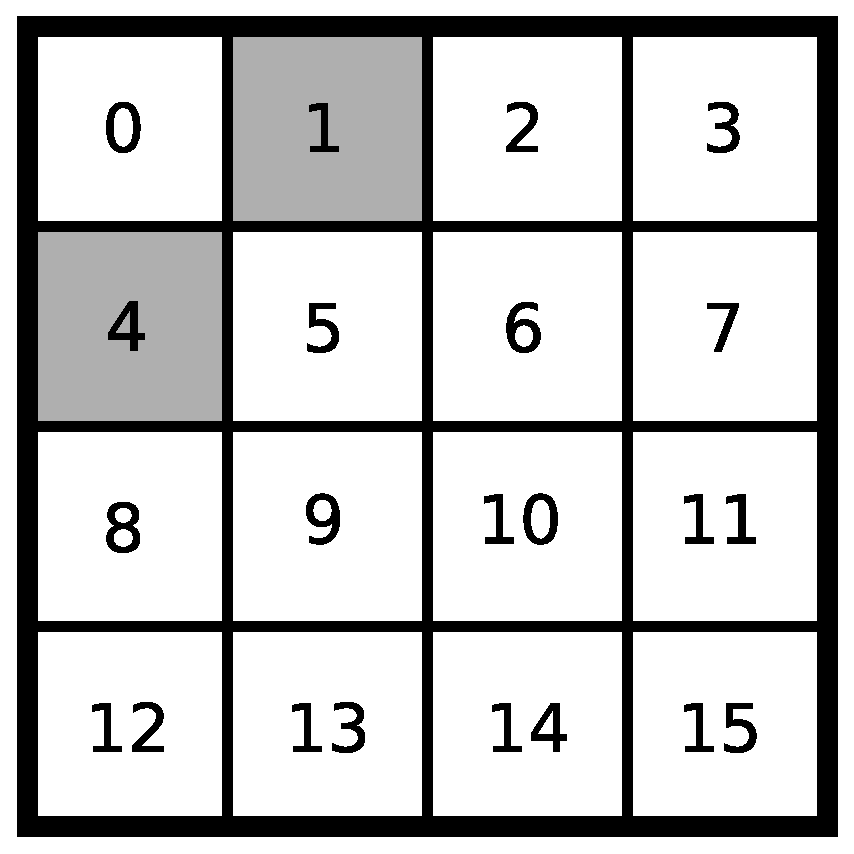
\includegraphics[width=2in]{images/duplicate-detection-scope.eps}
\caption{The abstract image of all states with a empty tile in the
  upper left corner (top) and the duplicate detection scope of this
  abstract node (bottom).}
\label{fig:tile-abstraction}
\end{center}
\end{figure}

This idea can be shown using the sliding tile puzzle as an example.
It is conceivable that a projection function for the sliding tiles
puzzle would be to only look at the position of the empty tile.  For
example: all states with the empty tile in the upper left-hand corner
(position 0) would map to the abstract state shown on the top in
Figure \ref{fig:tile-abstraction}, where the grayed tile represents
the position of the empty tile.  Using this abstraction, there are
sixteen possible abstract states.  It is easy to see that all of the
children of a state with the empty tile in position 0 will have the
empty tile in either position 1 or 4 (the abstract states with the
empty tile in position 1 or 4 are the successors of the abstract state
with the empty tile in position 0).  This means that when checking if
a child state (of a state in the nblock with the empty tile in
position 0) has already been generated, only the states in the nblocks
with the empty tile in position 1 and 4 need to be checked.  This is
the duplicate detection scope of the nblock with the empty tile in
position 0 (shown on the bottom in Figure \ref{fig:tile-abstraction}).

In \cite{zhou:sdd} Zhou and Hansen are interested in state-space
decomposition so that they can efficiently move generated nodes to a
secondary storage device (such as a disk drive).  The SDD approach
uses breadth-first heuristic search, and one nblock is searched at a
time.  Since duplicates can only lie in the duplicate detection scope
of the nblock being searched, the remainder of the nodes can be pushed
off to disk, instead of being stored in main memory.  Nblocks can then
be swapped into and out of main-memory as the search progresses.

\subsection{Parallel Structured Duplicate Detection (PSDD)}

While the motivation of SDD is to have explicit control of which
portions of a search space reside in main-memory (and which reside on
disk), in \cite{zhou:psd} Zhou and Hansen show that this approach
lends itself to parallelization.  The parallel SDD (or PSDD) approach
uses the graph of nblocks to find \emph{disjoint duplicate detection
  scopes}, or duplicate detection scopes that do not overlap.  Nblocks
with disjoint duplicate detection scopes can be searched in parallel
with out contention.  In fact, with PSDD, only a single shared
data structure is used, and this is the nblock graph which is used to
find free nblocks (that is, nblocks where no nblocks in their
duplicate detection scope are in use by another processor).  Once a
free nblock is acquired processor the nblock, and all of the nblocks
in its duplicate detection scope are no longer free, and the processor
can expand all of the nodes in the nblock without any locking or
waiting.

In PSDD, as in SDD, the search progresses in layers, in a
breadth-first manor.  For example, an nblock can be thought of as a
closed-list and two open-lists -- one for the current layer (which is
being expanded from) and one for the next layer (which is expanded
into).  Nodes are removed from the open-list of the current layer in
one nblock, duplicate detection is performed from the closed list of
the nblock of the child node, then (if the child is not a duplicate)
it is inserted into the next layer's open-list of its nblock.  When
the current layer of an nblock is done expanding, it is added to the
free nblock list of the next layer, and the processor tries to acquire
a new free nblock.  Once there are no more nblocks to expand on the
current layer, processors switch to the next layer and begin searching
again.  The search progresses in this fashion until a goal is found or
the entire search space is covered and there is no solution.  Since
the search order is breadth-first, the first goal that is found is the
optimal goal.

\section{Parallel Best NBlock First (PBNF)}
\subsection{Safe PBNF}
\section{Experimental Results}
\section{Conclusion}

\bibliography{master}
\bibliographystyle{aaai}

\end{document}
